% Options for packages loaded elsewhere
\PassOptionsToPackage{unicode}{hyperref}
\PassOptionsToPackage{hyphens}{url}
\PassOptionsToPackage{dvipsnames,svgnames,x11names}{xcolor}
%
\documentclass[
  letterpaper,
  DIV=11,
  numbers=noendperiod]{scrartcl}

\usepackage{amsmath,amssymb}
\usepackage{iftex}
\ifPDFTeX
  \usepackage[T1]{fontenc}
  \usepackage[utf8]{inputenc}
  \usepackage{textcomp} % provide euro and other symbols
\else % if luatex or xetex
  \usepackage{unicode-math}
  \defaultfontfeatures{Scale=MatchLowercase}
  \defaultfontfeatures[\rmfamily]{Ligatures=TeX,Scale=1}
\fi
\usepackage{lmodern}
\ifPDFTeX\else  
    % xetex/luatex font selection
\fi
% Use upquote if available, for straight quotes in verbatim environments
\IfFileExists{upquote.sty}{\usepackage{upquote}}{}
\IfFileExists{microtype.sty}{% use microtype if available
  \usepackage[]{microtype}
  \UseMicrotypeSet[protrusion]{basicmath} % disable protrusion for tt fonts
}{}
\makeatletter
\@ifundefined{KOMAClassName}{% if non-KOMA class
  \IfFileExists{parskip.sty}{%
    \usepackage{parskip}
  }{% else
    \setlength{\parindent}{0pt}
    \setlength{\parskip}{6pt plus 2pt minus 1pt}}
}{% if KOMA class
  \KOMAoptions{parskip=half}}
\makeatother
\usepackage{xcolor}
\setlength{\emergencystretch}{3em} % prevent overfull lines
\setcounter{secnumdepth}{-\maxdimen} % remove section numbering
% Make \paragraph and \subparagraph free-standing
\ifx\paragraph\undefined\else
  \let\oldparagraph\paragraph
  \renewcommand{\paragraph}[1]{\oldparagraph{#1}\mbox{}}
\fi
\ifx\subparagraph\undefined\else
  \let\oldsubparagraph\subparagraph
  \renewcommand{\subparagraph}[1]{\oldsubparagraph{#1}\mbox{}}
\fi


\providecommand{\tightlist}{%
  \setlength{\itemsep}{0pt}\setlength{\parskip}{0pt}}\usepackage{longtable,booktabs,array}
\usepackage{calc} % for calculating minipage widths
% Correct order of tables after \paragraph or \subparagraph
\usepackage{etoolbox}
\makeatletter
\patchcmd\longtable{\par}{\if@noskipsec\mbox{}\fi\par}{}{}
\makeatother
% Allow footnotes in longtable head/foot
\IfFileExists{footnotehyper.sty}{\usepackage{footnotehyper}}{\usepackage{footnote}}
\makesavenoteenv{longtable}
\usepackage{graphicx}
\makeatletter
\def\maxwidth{\ifdim\Gin@nat@width>\linewidth\linewidth\else\Gin@nat@width\fi}
\def\maxheight{\ifdim\Gin@nat@height>\textheight\textheight\else\Gin@nat@height\fi}
\makeatother
% Scale images if necessary, so that they will not overflow the page
% margins by default, and it is still possible to overwrite the defaults
% using explicit options in \includegraphics[width, height, ...]{}
\setkeys{Gin}{width=\maxwidth,height=\maxheight,keepaspectratio}
% Set default figure placement to htbp
\makeatletter
\def\fps@figure{htbp}
\makeatother

\KOMAoption{captions}{tableheading}
\makeatletter
\@ifpackageloaded{caption}{}{\usepackage{caption}}
\AtBeginDocument{%
\ifdefined\contentsname
  \renewcommand*\contentsname{Table of contents}
\else
  \newcommand\contentsname{Table of contents}
\fi
\ifdefined\listfigurename
  \renewcommand*\listfigurename{List of Figures}
\else
  \newcommand\listfigurename{List of Figures}
\fi
\ifdefined\listtablename
  \renewcommand*\listtablename{List of Tables}
\else
  \newcommand\listtablename{List of Tables}
\fi
\ifdefined\figurename
  \renewcommand*\figurename{Figure}
\else
  \newcommand\figurename{Figure}
\fi
\ifdefined\tablename
  \renewcommand*\tablename{Table}
\else
  \newcommand\tablename{Table}
\fi
}
\@ifpackageloaded{float}{}{\usepackage{float}}
\floatstyle{ruled}
\@ifundefined{c@chapter}{\newfloat{codelisting}{h}{lop}}{\newfloat{codelisting}{h}{lop}[chapter]}
\floatname{codelisting}{Listing}
\newcommand*\listoflistings{\listof{codelisting}{List of Listings}}
\makeatother
\makeatletter
\makeatother
\makeatletter
\@ifpackageloaded{caption}{}{\usepackage{caption}}
\@ifpackageloaded{subcaption}{}{\usepackage{subcaption}}
\makeatother
\ifLuaTeX
  \usepackage{selnolig}  % disable illegal ligatures
\fi
\usepackage{bookmark}

\IfFileExists{xurl.sty}{\usepackage{xurl}}{} % add URL line breaks if available
\urlstyle{same} % disable monospaced font for URLs
\hypersetup{
  pdftitle={591 Presentation},
  pdfauthor={Moses Farley},
  colorlinks=true,
  linkcolor={blue},
  filecolor={Maroon},
  citecolor={Blue},
  urlcolor={Blue},
  pdfcreator={LaTeX via pandoc}}

\title{591 Presentation}
\author{Moses Farley}
\date{}

\begin{document}
\maketitle

\subsection{Inspiration}\label{inspiration}

\href{https://www.mdpi.com/1999-4893/16/3/139}{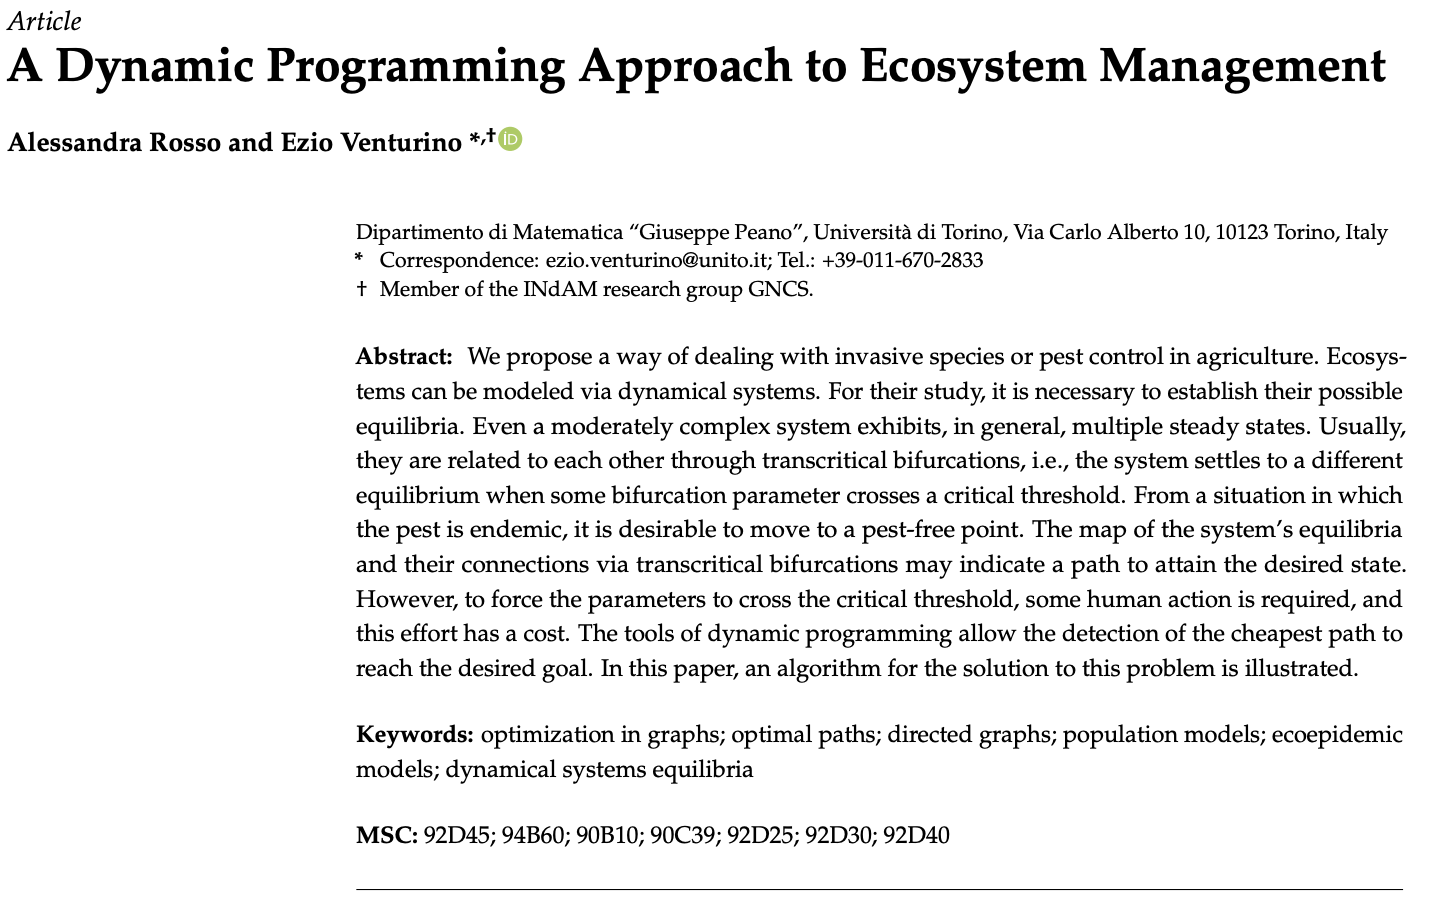
\includegraphics{images/dp_ecosystem.png}}

\subsection{Term 1: Dynamic Systems}\label{term-1-dynamic-systems}

\begin{itemize}
\item
  Definition: Systems that change over time, influenced by internal and
  external factors
\item
  Ecological Relevance: Interconnected components of ecosystems
  (e.g.~populations, resources, climate, etc\ldots)
\item
  Key components:

  \begin{itemize}
  \item
    Non-linearity: Small changes can lead to large effects
  \item
    Feedback loops: Interactions between components can amplify or
    dampen changes
  \item
    Emergent properties: complex patterns arise from simple interactions
  \end{itemize}
\end{itemize}

\subsection{Term 2: Transcritical
Bifurcation}\label{term-2-transcritical-bifurcation}

\begin{itemize}
\item
  Two states exist (one is stable, the other is unstable).
\item
  A smooth change in a parameter causes them to swap stability. Imagine
  the ``smooth change'' as a turning a knob.
\item
  Really simplified definition without getting in differential
  equations, eigenvalues (I'm not able to cover lol)
\end{itemize}

\subsection{Term 2: Example using {[}blank{]}
populations}\label{term-2-example-using-blank-populations}

\begin{itemize}
\tightlist
\item
  State A: low population \& State B: high population
\item
  Before the switch (low knob setting): State A is stable and the
  population tends to stay low.

  \begin{itemize}
  \tightlist
  \item
    State B is unstable - if the population gets too high, something
    (like lack of food) will cause it to crash back down.
  \end{itemize}
\item
  After the switch (high knob setting): State B is now stable - the
  population tends to stay high.

  \begin{itemize}
  \tightlist
  \item
    State A is now unstable - if the population gets too low, something
    (like random deaths) could wipe it out completely.
  \end{itemize}
\item
  As you gradually increase the knob setting (maybe by introducing more
  food), the two populations ``switch places'' in terms of their
  stability.
\end{itemize}

\subsection{Term 3: Graph (Network)}\label{term-3-graph-network}

\begin{itemize}
\tightlist
\item
  A \textbf{graph} is a collection of \textbf{nodes} (vertices)
  connected by \textbf{edges} (links), where each edge has an associated
  \textbf{weight} (cost or distance). For my use (via the Bellman-Ford
  algorithm), the graph can be directed, and edge weights may be
  negative, enabling the algorithm to find the shortest path from a
  single source node to all other nodes, even in graphs with negative
  weights (but no negative weight cycles).
\end{itemize}

\subsection{Network Flow Example}\label{network-flow-example}

\begin{figure}[H]

{\centering \includegraphics[width=8.25in,height=\textheight]{images/Shortest_path_Dijkstra_vs_BellmanFord.gif}

}

\caption{Shortest path Dijkstra vs Bellman-Ford Algorithms}

\end{figure}%

\subsection{Rodents, Foxes, and
parasites}\label{rodents-foxes-and-parasites}

\begin{figure}[H]

{\centering 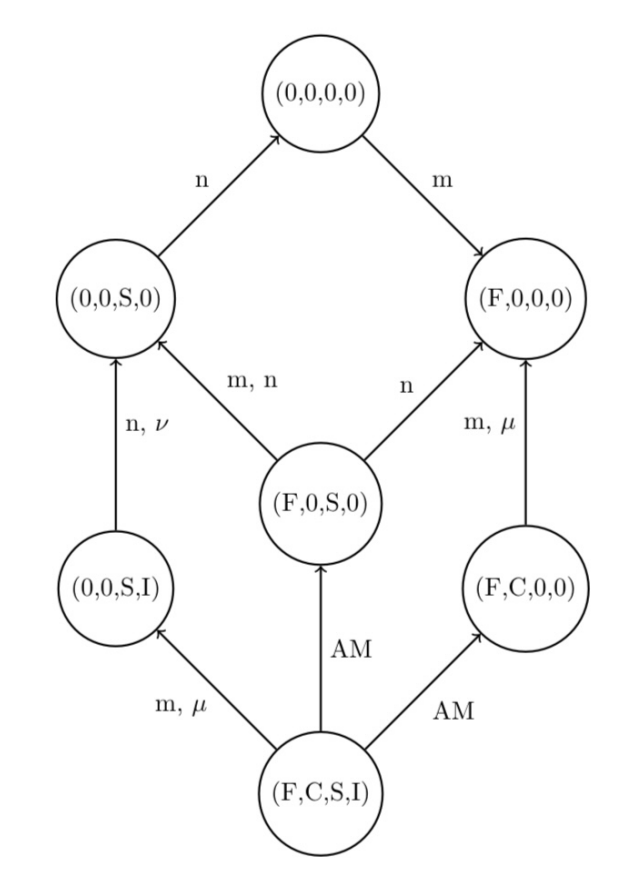
\includegraphics[width=4.16667in,height=\textheight]{images/DP_foxes.png}

}

\caption{Figure 1. The graph of the equilibria for system (1) and the
transcritical bifurcations relating them.}

\end{figure}%

Healthy foxes F, healthy rodents S, infected foxes C and infected
rodents I populations, AM is dependency on all four mortality parameters
(0 represent erradication). Natural and disease-induced mortalities, m,
n, µ, ν for healthy foxes and rodents, and infected foxes and rodents,
respectively.

\subsection{Path-finding Example}\label{path-finding-example}

\begin{figure}[H]

{\centering 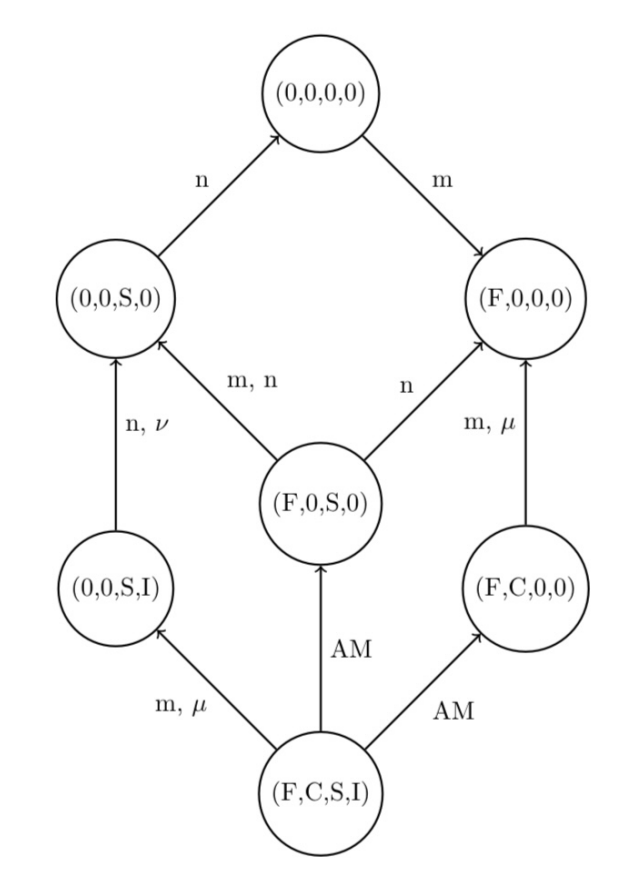
\includegraphics[width=4.16667in,height=\textheight]{images/DP_foxes.png}

}

\caption{Figure 1. The graph of the equilibria for system (1) and the
transcritical bifurcations relating them.}

\end{figure}%

\begin{figure}[H]

{\centering 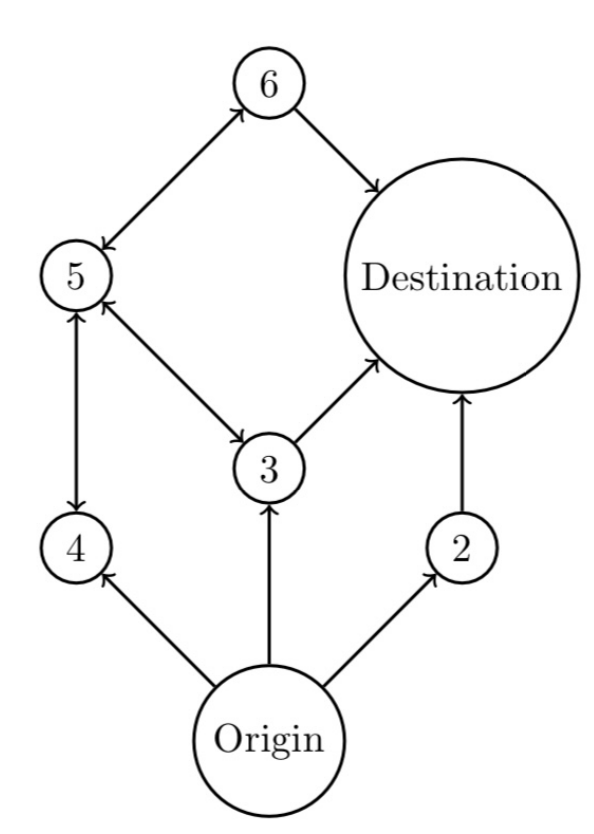
\includegraphics[width=4.16667in,height=\textheight]{images/fox_dest.png}

}

\caption{Parasite and Rodent Free Equilibrium}

\end{figure}%

\begin{figure}[H]

{\centering 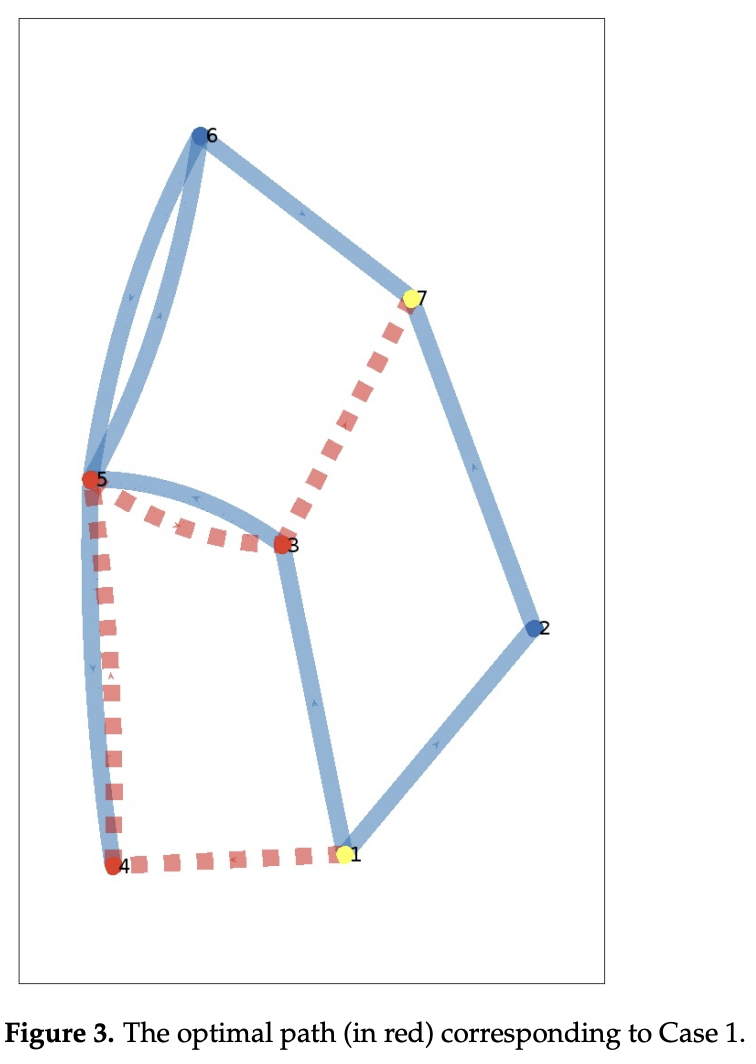
\includegraphics[width=4.16667in,height=\textheight]{images/fox_path.png}

}

\caption{Figure 3. The optimal path (in red) corresponding to Parasite
and Rodent Free}

\end{figure}%

\subsection{Applications for Moses \& Applied
Ecology}\label{applications-for-moses-applied-ecology}

Analysis of invasive mutualism?

\begin{itemize}
\item
  Spotted lantern fly and Ailanthus
\item
  Fig trees and wasps
\item
  Fir trees and fungus
\end{itemize}

\subsection{Needs for me (improvement)}\label{needs-for-me-improvement}

\begin{itemize}
\item
  Better understanding of bifurcation theory\textbackslash differential
  equations

  \begin{itemize}
  \item
    Equation crucial to the Dynamic Programming aspect is mass action
    disease incidence (homogeneous populations mixing) equation.
  \item
    \begin{figure}[H]

    {\centering 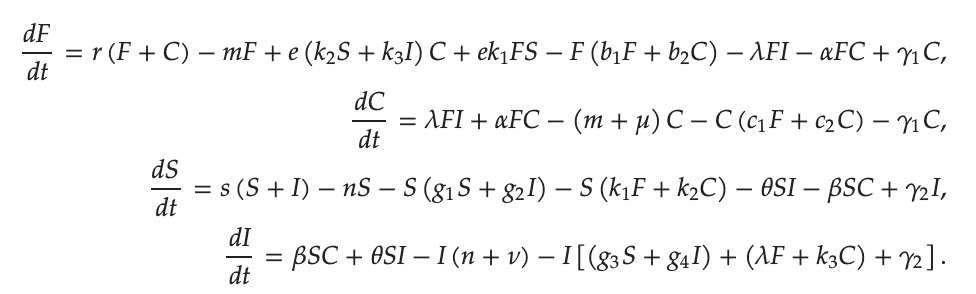
\includegraphics[width=4.65625in,height=\textheight]{images/equation.png}

    }

    \caption{Mass action disease incidence}

    \end{figure}%
  \end{itemize}
\item
  Better background on how to obtain sample data (no data availability
  for Torino study)
\item
  Figuring out locations, costs and attainable time windows.
\item
  Follow directions!
\end{itemize}

\subsection{Sources}\label{sources}

\begin{enumerate}
\def\labelenumi{\arabic{enumi}.}
\tightlist
\item
  Rosso, A.; Venturino, E. A Dynamic Programming Approach to Ecosystem
  Management. Algorithms 2023, 16, 139.
  https://doi.org/10.3390/a16030139
\item
  Rosso, A.; Venturino, E. Comparison of two mathematical models for the
  Echinococcus multilocularis-red foxes-rodents interactions. Algorithms
  2021. https://repositorio.utem.cl/handle/30081993/1172
\item
  Empirical dynamic programming for model-free ecosystem-based
  management.
  \href{https://doi.org/10.1111/2041-210X.14302}{\textbf{https://doi.org/10.1111/2041-210X.14302}}
\item
  Yakowitz, S. Dynamic programming applications in water resources.
  Water Resour. Res. 1982, 18, 673--696.
\end{enumerate}



\end{document}
